\documentclass[xcolor=table]{beamer}
\usepackage{lmodern}
%\usepackage[normalem]{ulem}
\usepackage{ marvosym }
\usepackage[export]{adjustbox}
\usepackage{mathtools,calc}
\newcommand\Fontvi{\fontsize{22}{23.2}\selectfont}
\newcommand\strikeout[2][]{%
 \begin{tabular}[b]{@{}c@{}}
    \makebox(0,0)[cb]{\textcolor{blue}{#1}} \\[-0.2\normalbaselineskip]
     \rlap{\color{red}\rule[0.5ex]{\widthof{#2}}{0.5pt}}#2
 \end{tabular}}

\newcommand<>\mathalt[2]{%
  \alt#3{\mathmakebox[\widthof{$#2$}]{#1}}{#2}%
}
\usepackage{colortbl}
\usepackage{minted}
\usepackage{booktabs}
%\usepackage{xcolor}
%\usepackage[usenames, dvipsnames]{color}
\definecolor{red}{rgb}{0.894, 0.101, 0.109} 
\definecolor{Gray}{gray}{0.85}
\newcolumntype{a}{>{\columncolor{Gray}}c}
\definecolor{green}{rgb}{0.1054, 0.6171, 0.4648}
\definecolor{orange}{rgb}{0.8476, 0.3711, 0.0078}
\definecolor{violet}{rgb}{0.9023, 0.1602, 0.5391}
%\usepackage[doi=false, backref=true, url=false, isbn=false, backend=biber,
						%citestyle=authoryear]{biblatex}
\usepackage{tabu}
\newcommand{\blue}{\textcolor{blue}}
\newcommand{\red}{\textcolor{red}}
\newcommand{\green}{\textcolor{green}}
\newcommand{\organge}{\textcolor{orange}}
\newcommand{\violet}{\textcolor{violet}}
% Just for demo

\AtBeginSection[]{
  \begin{frame}
  \vfill
  \centering
  \begin{beamercolorbox}[sep=8pt,center,shadow=true,rounded=true]{title}
    \usebeamerfont{title}\insertsectionhead\par%
  \end{beamercolorbox}
  \vfill
  \end{frame}
}
\usepackage{mathtools}
\newtheorem{prop}{Proposition}
\newtheorem{hypothesis}{Hypothesis}
\usepackage{amsmath}
\usepackage{multirow}
\usepackage{makecell} % to make linebreaks in table
\renewcommand\theadalign{bc}
\renewcommand\theadfont{\bfseries}
\renewcommand\theadgape{\Gape[4pt]}
\renewcommand\cellgape{\Gape[4pt]}
\usepackage{hhline}
\usepackage{geometry}
\usepackage{booktabs}
\usepackage[]{hyperref}%
\hypersetup{colorlinks, linkcolor={blue}, citecolor={blue}, urlcolor={red}}
\usepackage{graphicx}

\DeclareMathOperator*{\argmax}{\arg\!\max}
\DeclareMathOperator{\E}{\mathbb{E}}
%\addbibresource[]{library.bib}
\usepackage[utf8]{inputenc}
\usepackage[T1]{fontenc}
\setbeamertemplate{caption}{\raggedright\insertcaption\par}
\usetheme{default}
\usepackage[flushleft]{threeparttable}
\usepackage{booktabs,caption,fixltx2e}
\usepackage{ragged2e}
\usepackage{appendixnumberbeamer}
\makeatletter
\usefonttheme{professionalfonts}
\usefonttheme{serif}
\setbeamertemplate{navigation symbols}{}%remove navigation symbols
\setbeamertemplate{footline}
{
  \leavevmode%
  \hbox{%
  \begin{beamercolorbox}[wd=.333333\paperwidth,ht=2.25ex,dp=1ex,center]{author in head/foot}%
    \usebeamerfont{author in head/foot}\insertsection\
  \end{beamercolorbox}%
  \begin{beamercolorbox}[wd=.333333\paperwidth,ht=2.25ex,dp=1ex,center]{title in head/foot}%
    \usebeamerfont{title in head/foot}\insertsubsection\
  \end{beamercolorbox}%
  \begin{beamercolorbox}[wd=.333333\paperwidth,ht=2.25ex,dp=1ex,right]{date in head/foot}%
    %\usebeamerfont{date in head/foot}\insertshortdate{}\hspace*{2em} % hide %date
    %\insertframenumber{} / \inserttotalframenumber\hspace*{2ex} 
  \end{beamercolorbox}}%
  \vskip0pt%
}
\makeatother
%\setbeamertemplate{footline}[frame number]{}


\usepackage{listings}
\lstset{
    tabsize=4,
    showstringspaces=false,
    numbers=left,
    commentstyle=\color{green},
    keywordstyle=\color{blue},
    stringstyle=\color{red}
}


 %----------------------------------------------------------------------------------------
% %	TITLE PAGE
% %----------------------------------------------------------------------------------------
\renewcommand*{\thefootnote}{\fnsymbol{footnote}}
\title[]{Mergesort with CUDA}
\date{25.02.2020} % Date, can be changed to a custom date
%\author{Fabian Schuetze, EUI}
\addtobeamertemplate{block begin}{}{\justifying}  %new code
\setbeamertemplate{itemize items}[circle]

\usepackage{tikz, enumitem}
\usetikzlibrary{positioning}% for positioning of nodes
\usetikzlibrary{decorations.pathreplacing,positioning, arrows.meta}
\newcommand{\ImageWidth}{11cm}


\begin{document}

\begin{frame}
\titlepage
\end{frame}

\begin{frame}
\tableofcontents
\end{frame}

\section{Architecture}

\begin{frame}[fragile]
\frametitle{GPU and CPU uses different memories}
\begin{figure}[ht]
   \centering
   \includegraphics[scale=0.7]{architecture.png}
\end{figure}
\green{Init:}
\begin{minted}[linenos=true]{cpp}
T* gpup;
int sz = 10*sizeof(int);
cudaMalloc((void**)&gpup, sz);
\end{minted}
\green{Memory Transfer:}
\begin{minted}[linenos=true]{cpp}
cudaMemcpy(gpup, cpup, nBytes, cudaMemcpyHostToDevice);
\end{minted}
\end{frame}

\begin{frame}[fragile]
\frametitle{Ideas for Memory Management}
\begin{minted}[linenos=true]{cpp}
class Storage {
   public:
    explicit Storage(const std::vector<T>&);

   private:
    std::vector<T> _data;
    T* _cpu_pointer;
    T* _gpu_pointer;
    void initialize_gpu_memory();
};
\end{minted}
\begin{itemize}
    \item Memory pool, takes ownership
    \item Initializes the gpu memory as copy
    \item Pointers for cpu/gpu locations
\end{itemize}
\end{frame}

\begin{frame}[fragile]
    \frametitle{Lazy Memory Sync}
\begin{minted}[linenos=true]{cpp}
class Storage {
   public:
    T* cpu_pointer();
    T* gpu_pointer();
    const T* cpu_pointer_const();
    const T* gpu_pointer_const();

   private:
    std::string head; \\ head = {CPU, GPU, SYNC}
    void sync_to_cpu();
    void sync_to_gpu();
};
\end{minted}
\green{Example:}
\begin{itemize}
    \item After Initialization: \mintinline{c++}{head = SYNC}
    \item Access, \mintinline{c++}{gpu_pointer_const(): head} remains
    \item Access \mintinline{c++}{cpu_pointer(): head = CPU}
    \item Acess \mintinline{c++}{gpu_pointer(): sync_to_cpu(); head = SYNC}
\end{itemize}
\end{frame}

\section{Mapping Cuda calls to Hardware}
\begin{frame}[fragile]
\frametitle{Launching CUDA threads}
\green{Cuda Program}
\begin{minted}[linenos=true]{cpp}
dim3 Grid(2)
dim3 Block(4)
add_kernel<<<Grid, Block>>>(...)
\end{minted}
    \green{Thread Layout:}
    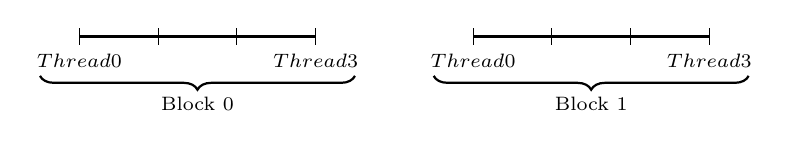
\begin{tikzpicture}
% draw horizontal line
\draw[thick,- ] (0,0) -- (3,0) node[font=\scriptsize,below left=3pt and
        -5pt]{};
\draw[thick,- ] (5,0) -- (8,0) node[font=\scriptsize,below left=3pt and
        -5pt]{};


% draw vertical lines
\foreach \x in {0,1,...,3}
\draw (\x cm,3pt) -- (\x cm,-3pt);

\foreach \x in {5,6,...,8}
\draw (\x cm,3pt) -- (\x cm,-3pt);

\foreach \x/\descr in {0/Thread 0,3/Thread 3}
\node[font=\scriptsize, text height=1.75ex,
text depth=.5ex] at (\x,-.3) {$\descr$};

\foreach \x/\descr in {5/Thread 0,8/Thread 3}
\node[font=\scriptsize, text height=1.75ex,
text depth=.5ex] at (\x,-.3) {$\descr$};

\draw [thick ,decorate,decoration={brace,amplitude=5pt}] (3.5,-0.5)  -- +(-4,0) 
       node [black,midway,below=4pt, font=\scriptsize] {Block 0};
\draw [thick ,decorate,decoration={brace,amplitude=5pt}] (8.5,-0.5)  -- +(-4,0) 
       node [black,midway,below=4pt, font=\scriptsize] {Block 1};
    \end{tikzpicture}
    \green{Addition:}
\begin{minted}[linenos=true]{cuda}
__global__ 
add_kernel(float* A, float* B, float* C, int n) {
    int i = blockDim.x * blockIdx.x + threadIdx.x;
    if (i < n) {
        C[i] = A[i] + B[i];
    }
}
\end{minted}
\end{frame}

\begin{frame}
\frametitle{Software/Hardware connection}
\green{Programmer:} Specifies number of blocks and threads
\begin{overlayarea}{\textwidth}{4.5cm}
\only<1, 3>{
\begin{figure}[ht]
   \centering
   \includegraphics[scale=0.25]{cuda_architecture.png}
\end{figure}
 }
\only<2,4>{
\begin{figure}[ht]
   \centering
   \includegraphics[scale=0.25]{sm_dispatch.png}
\end{figure}
}
\end{overlayarea}
    \begin{overlayarea}{\textwidth}{3.0cm}
\only<1->{
\red{Dispatch:\\}
\green{1. Blocks to SM:} Block 1 $\rightarrow$ SM1, Block 2 $\rightarrow$
    SM2 $\ldots$\\
}
\only<2->{
\green{2. Grouping:} Wrappend threads are allocated\\
}
\only<3->{
\red{Stengths:\\}
\green{Quantity: } No branch prediction/ chaches, just cores\\
}
\only<4->{
\green{Latency Hiding:} If wrap 1 stalls, scheduler starts wrap 2 
}
\end{overlayarea}
\end{frame}

\section{Merge}

\begin{frame}[fragile]
    \frametitle{Basic Merge Operation}
\begin{align*}
    A &= \begin{matrix} 5 & 7 & 8& & &  9&  12&  14&  15&  16 \end{matrix} \\
    B &= \begin{matrix} 1&  2&  3&  4&  6&  10&  11&  13 \end{matrix} \\
    C &= \begin{matrix} ?&  ?&  ?&  ?&  ?&  ?&  ?&  ?&  ?&  ?&  ?&  ?&
            ?& ?& ?& ? \end{matrix}
\end{align*}
\begin{minted}[linenos=true]{c++}
void merge(T* a, T* b, T* c, int sz_a, int sz_b) {
    int i = 0, j = 0, k = 0;
    while (k < sz_a + sz_b) {
        if (i == sz_a)
            c[k++] = b[j++];
        else if (j == sz_b)
            c[k++] = a[i++];
        else if (a[i] <= b[j])
            c[k++] = a[i++];
        else
            c[k++] = b[j++];
    }
}
\end{minted}
\green{Problem:} complexity, $\mathcal{O}(n)$
\end{frame}

\begin{frame}
\frametitle{How to split A and B to spwan many threads?}
\begin{overlayarea}{\textwidth}{10cm}
\only<1->{
\green{Example:}
\begin{align*}
    A &= \begin{matrix} 0 & 0&0&0 \end{matrix} \\
    B &= \begin{matrix} 1&1&1&1 \end{matrix} \\
    C &= \begin{matrix} ?&?&?&?&?&?&?&? \end{matrix}
\end{align*}
}
\only<2->{
\green{Naive:} 2 Threads, half A and B \\
\begin{align*}
    A &= \begin{matrix} \underbrace{0 & 0}_{\text{Thread 1}} | 
    \underbrace{0 & 0}_{\text{Thread 2}} \end{matrix} \\
    B &= \begin{matrix} \underbrace{1 & 1}_{\text{Thread 1}} | 
    \underbrace{1 & 1}_{\text{Thread 2}} \end{matrix} \\
    C &= \begin{matrix} \underbrace{? &?& ?& ?}_{\text{Thread 1}} | 
    \underbrace{?& ?& ?& ?}_{\text{Thread 2}} \end{matrix}
\end{align*}
}
\only<3->{
\green{Result:}
\begin{align*}
    C &= \begin{matrix} \underbrace{0& 0& 1& 1}_{\text{Thread 1}} | 
    \underbrace{0& 0& 1& 1}_{\text{Thread 2}} \end{matrix}
\end{align*}
}
\end{frame}

\begin{frame}
\frametitle{Instead: How to split arrays}
NEED TO CITE PAPER!
\begin{overlayarea}{\textwidth}{5.0cm}
\only<1>{
   \begin{figure}[ht]
       \centering
       \textbf{How to split two arrays in equal chuncks?}
       \includegraphics[scale=0.17]{initial.png}
    \end{figure}
 }
\only<2>{
   \begin{figure}[ht]
   \centering
       \textbf{One feasible split: Array A to Thread 1, Array B to Thread 2}
   \includegraphics[scale=0.17]{feasible_1.png}
    \end{figure}
 }
\only<3>{
   \begin{figure}[ht]
   \centering
   \textbf{Another feasible split: Array B to Thread 1, Array A to Thread 2}
   \includegraphics[scale=0.17]{feasible_2.png}
    \end{figure}
 }
\only<4>{
   \begin{figure}[ht]
   \centering
   \textbf{Another split (seen before): Thread 1 gets half of A and B}
   \includegraphics[scale=0.17]{feasible_3.png}
    \end{figure}
    \red{Summary:} All allocations along vertical line split work equally!
 }
\only<5>{
   \begin{figure}[ht]
   \centering
   \textbf{Mergepath: Define the optimal split: One Elemet of B}
   \includegraphics[scale=0.17]{mergepath_1.png}
    \end{figure}
    \red{Summary:} All allocations along vertical line split work equally!
    \green{Mergpath:} Vertical move: pick array B; horizontal move: Array
 }
\only<6>{
   \begin{figure}[ht]
   \centering
   \textbf{Mergepath: Define the optimal split: Another Elemet of B}
   \includegraphics[scale=0.17]{mergepath_2.png}
    \end{figure}
 }
\only<7>{
   \begin{figure}[ht]
   \centering
   \textbf{Mergepath: Define the optimal split: Another Elemet of B}
   \includegraphics[scale=0.17]{mergepath_3.png}
    \end{figure}
 }
\only<8>{
   \begin{figure}[ht]
   \centering
   \textbf{Mergepath: Define the optimal split: Another Elemet of B}
   \includegraphics[scale=0.17]{mergepath_4.png}
    \end{figure}
 }
\only<9>{
   \begin{figure}[ht]
   \centering
   \textbf{Mergepath: Define the optimal split: Pick first elment of A}
   \includegraphics[scale=0.17]{mergepath_5.png}
    \end{figure}
 }
\only<10>{
   \begin{figure}[ht]
   \centering
   \includegraphics[scale=0.17]{mergepath_6.png}
    \end{figure}
 }
\only<11>{
   \begin{figure}[ht]
   \centering
   \includegraphics[scale=0.17]{mergepath_7.png}
    \end{figure}
 }
\end{overlayarea}
\end{frame}

\begin{frame}[fragile]
\frametitle{Computation Procedure}
\begin{minted}[linenos=true]{cuda}
__global__ 
void paralleMerge(int* a, int sz_a, int* b, int sz_b, 
                  int* c, int length)
{
    int diag = threadIdx.x * length;
    int a_start = mergepath(a, sz_a, b, sz_b, diag);
    int b_start = diag - a_start;
    merge(a, a_start, sz_a, b, b_start, sz_b, c, diag, length);
}
\end{minted}
\begin{itemize}
    \item Each tread works on one part
    \item Thread calculates \mintinline{c++}{$A_lower$} \mintinline{c++}{mergepath}
    \item Obtain \mintinline{c++}{B_lower} as difference
    \item merges two sub-arrays
\end{itemize}
\end{frame}


\begin{frame}
\frametitle{Problem: Slow as a Snail}
\begin{figure}[ht]
\centering
\includegraphics[scale=0.25]{global_memory_merge.png}
\end{figure}
\end{frame}

\begin{frame}
\frametitle{Reason: So much global meory access}
\begin{overlayarea}{\textwidth}{5.0cm}
\only<1>{
\begin{figure}[ht]
\centering
\includegraphics[scale=0.25]{memory_access_pattern_1.png}
\end{figure}
}
\only<2>{
\begin{figure}[ht]
\centering
\includegraphics[scale=0.25]{memory_access_pattern_3.png}
\end{figure}
}
\end{overlayarea}
\end{frame}

\section{Memory Hirachy of CUDA}
\begin{frame}
\frametitle{The different memories and their sizes}
\begin{figure}[ht]
\centering
\includegraphics[scale=0.22]{memory_hirachy.png}
\end{figure}
\red{Visibility:}
\begin{itemize}
    \item \green{Global Memory:} Accessed by all threads\\
    \item \green{Shared Memory:} Private for Block\\
    \itme \green{Registers:} Private for Thread\\
\end{itemize}
\red{Size:}
\begin{itemize}
    \item \green{Global Memory:} 2 GB
    \item \green{Shared Memory:} Total: 192 KB, per block: 48 KB
\end{itemize}
\red{Latency:}
\begin{itemize}
    \item \green{Global Memory:} 8 GB/s
    \item \green{Shared Memory:} 80 GB/s
\end{itemize}
\end{frame}

\section{Merging with local memory}
\begin{frame}
\frametitle{General Idea}
\red{Problem:} Block shared memory:  48 Kb -> need to make blocks small enough
\red{Solution:}
\begin{enumerate}
    \item Determine large but small enough chuncks of arrays to load into blocks
    \item Load into shared memeory
    \item Each thread determines its range (as before), from shared memory
    \item Each thread merges subset (as before)
\end{enumerate}
\end{frame}

\begin{frame}
\begin{minted}[lineos=true]{cuda}
__global__ void paralleMerge(const int* a, int sz_a, const int* b, int sz_b,
                             int* c, int* boundaries, int length,
                             int size_shared) {
    extern __shared__ int shared[];
    __shared__ int block_ranges[4];
    ranges(block_ranges, sz_a, sz_b, boundaries);
    loadtodevice(a, sz_a, b, sz_b, block_ranges, shared);
    //int process = threadIdx.x;
    int diag = threadIdx.x * length;
    if (diag < block_ranges[2] + block_ranges[3]) {
        int a_start =
            mergepath(shared, block_ranges[2], &shared[block_ranges[2]],
                      block_ranges[3], diag);
        int b_start = diag - a_start;
        merge(shared, a_start, block_ranges[2], &shared[block_ranges[2]],
              b_start, block_ranges[3], c, diag + blockIdx.x * size_shared,
              length);
    }
}
\end{minted}
\end{frame}

\begin{frame}
\frametitle{Show the results}
\begin{figure}[ht]
\centering
\includegraphics[scale=0.22]{shared_memory_merge.png}
\end{figure}
\end{frame}
\end{document}
